\documentclass[12pt,a4paper]{article}
\usepackage[latin1]{inputenc}
\usepackage[brazil]{babel}
\usepackage{amsmath}
\usepackage{amsfonts}
\usepackage{amssymb}
\usepackage{graphicx}
\usepackage[top=2cm, bottom=2cm, left=3cm, right=2cm]{geometry}
\author{Leonardo Amorim - 15/0039921}
\title{\textbf{Teste 9 - Soma do quadrado de dois n�meros de 4 bits}}
\date{}
\begin{document}
\maketitle

	 
\textbf{Funcionamento do c�digo}: Este programa em assembly tem o objetivo de somar dois n�meros de quatro 
bits elevados ao quadrado, da forma $a^2 + b^2$. O programa principal possui uma ordem de rotinas da forma mostrada na figura \ref{fig:rotinas}. A sequ�ncia de a��es a serem realizadas no c�digo se definem em limpar os dados de mem�ria (realizado ao iniciar o programa pela primeira vez), ler os dados das chaves, elevar ao quadrado, escrever no led e retornar a ler os dados das chaves, continuando o loop.


\begin{figure}[!htb]
	\centering
	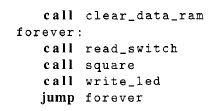
\includegraphics[scale=1.0]{rotinas.jpg}
	\caption{Forma de como as rotinas foram organizadas}
	\label{fig:rotinas}
\end{figure}

	 Uma parte do c�digo utilizado pode ser visualizado na figura \ref{fig:codigo}.

\begin{figure}[h]
	\centering
	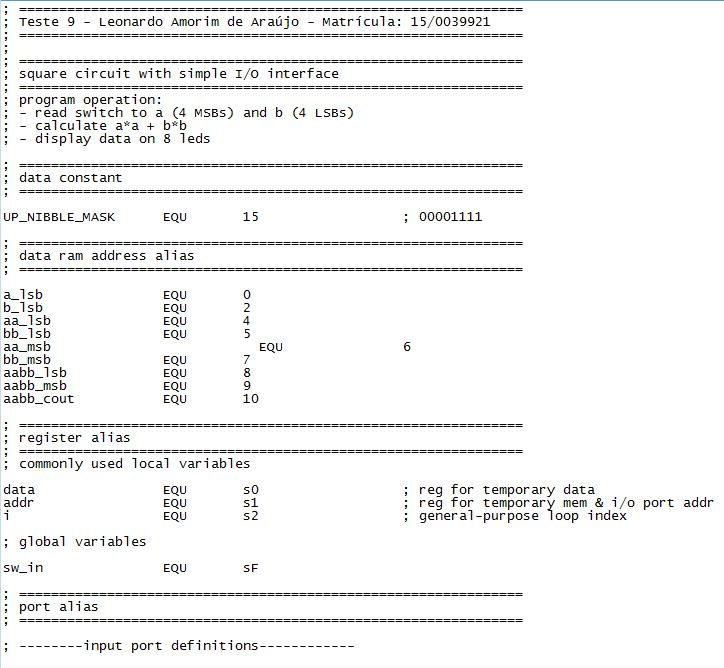
\includegraphics[scale=0.7]{codigo.jpg}
	\caption{C�digo utilizado}
	\label{fig:codigo}
\end{figure}

	 Abaixo segue uma amostra do funcionamento do c�digo. Neste momento est� sendo realizado a primeira multiplica��o do n�mero $a\times a$. Isto pode ser visto na figura \ref{fig:simulacao1}. 

\begin{figure}[h]
	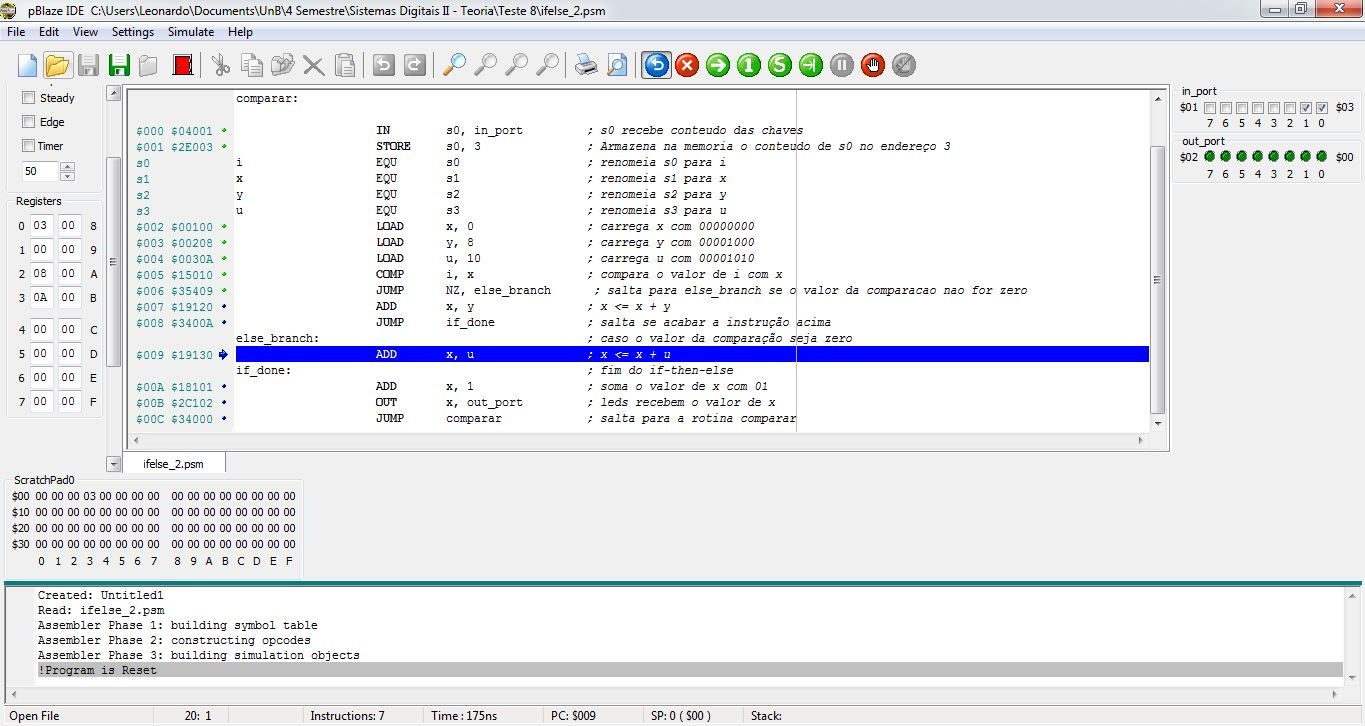
\includegraphics[scale=0.45]{simulacao1.jpg}
	\caption{Simula��o do c�digo}
	\label{fig:simulacao1}
\end{figure}

	\item Na figura \ref{fig:simulacao2} pode ser visto o resultado da opera��o $2^2 + 1^2 = 5 $, ao qual o valor aparece nos leds corretamente.

\begin{figure}[h]
	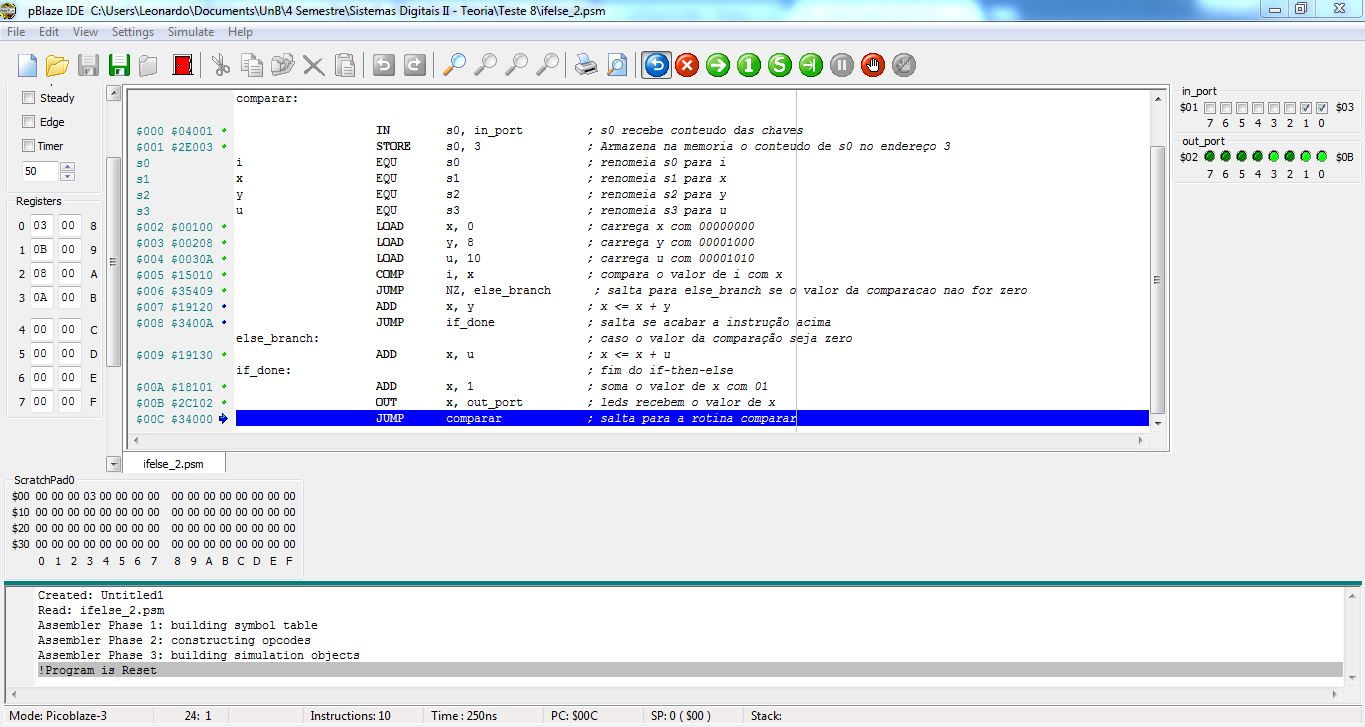
\includegraphics[scale=0.45]{simulacao2.jpg}
	\caption{Simula��o do c�digo - Resultado do uso dos dois n�meros da matr�cula 15/0039921}
	\label{fig:simulacao2}
\end{figure}

\end{document}